In this section, we present and discuss additional investigations into the stability of our models, expanding upon the discussion in Section~\ref{sec:analysis}.

% \subsection{Is collapse unavoidable?}
\subsection{Intervening Before Collapse}
% \subsection{Can One Intervene to Prevent Collapse?}
The symptoms of collapse are sharp and sudden, with sample quality dropping from its peak to its lowest value over the course of a few hundred iterations. We can detect this collapse when the singular values in \gen{} explode, but while the (unnormalized) singular values grow throughout training, there is no consistent threshold at which collapse occurs. This raises the question of whether it is possible to prevent or delay collapse by taking a model checkpoint several thousand iterations before collapse, and continuing training with some hyperparameters modified (e.g., the learning rate).

We conducted a range of intervention experiments wherein we took checkpoints of a collapsed model ten or twenty thousand iterations before collapse, changed some aspect of the training setup, then observed whether collapse occurred, when it occurred relative to the original collapse, and the final performance attained at collapse.

We found that increasing the learning rates (relative to their initial values) in either \gen{} or \discr{}, or both \gen{} and \discr{},  led to immediate collapse. This occurred even when doubling the learning rates from $2\cdot10^{-4}$ in \discr{} and $5\cdot10^{-5}$ in \gen{}, to $4\cdot10^{-4}$ in \discr{} and $1\cdot10^{-4}$ in \gen{}, a setting which is not normally unstable when used as the initial learning rates. We also tried changing the momentum terms (Adam's $\beta_1$ and $\beta_2$), or resetting the momentum vectors to zero, but this tended to either make no difference or, when increasing the momentum, cause immediate collapse.


We found that decreasing the learning rate in \gen{}, but keeping the learning rate in \discr{} unchanged could delay collapse (in some cases by over one hundred thousand iterations), but also crippled training---once the learning rate in \gen{} was decayed, performance either stayed constant or slowly decayed. Conversely, reducing the learning rate in \discr{} while keeping \gen{}'s learning rate led to immediate collapse. We hypothesize that this is because of the need for \discr{} to remain optimal throughout training---if its learning rate is reduced, it can no longer ``keep up" with \gen{}, and training collapses. With this in mind, we also tried increasing the number of \discr{} steps per \gen{} step, but this either had no effect, or delayed collapse at the cost of crippling training (similar to decaying \gen{}'s learning rate).


%...Suggests the training dynamics of our models are in some sense attuned to their optimization hyperparameters, and changing those hyperparameters partway through training encourages unfavorable dynamics...

%...One possible explanation is that as the singular values grow, the model draws close to the point of collapse and as they get larger the probability of total collapse approaches 1, and all it takes is a small perturbation to knock everything over...

To further illuminate these dynamics, we construct two additional intervention experiments, one where we freeze \gen{} before collapse (by ceasing all parameter updates) and observe whether \discr{} remains stable, and the reverse, where we freeze \discr{} before collapse and observe whether \gen{} remains stable. We find that when \gen{} is frozen, \discr{} remains stable, and slowly reduces both components of its loss towards zero. However, when \discr{} is frozen, \gen{} immediately and dramatically collapses, maxing out \discr{}'s loss to values upwards of 300, compared to the normal range of 0 to 3. 

%Regardless of \gen{}'s conditioning or optimization settings, the consequence of \gen{} being allowed to win the game is a complete breakdown of the training process.


This leads to two conclusions: first, as has been noted in previous works \citep{miyato2018spectral, gulrajani2017improved, zhang2018sagan}, \discr{} must remain optimal with respect to \gen{} both for stability and to provide useful gradient information. The consequence of \gen{} being allowed to win the game is a complete breakdown of the training process, regardless of \gen{}'s conditioning or optimization settings. Second, favoring \discr{} over \gen{} (either by training it with a larger learning rate, or for more steps) is insufficient to ensure stability even if \discr{} is well-conditioned. This suggests either that in practice, an optimal \discr{} is necessary but insufficient for training stability, or that some aspect of the system results in \discr{} not being trained towards optimality. With the latter possibility in mind, we take a closer look at the noise in \discr{}'s spectra in the following section.

%Second, if collapse occurs because of a failure of \discr{}, providing \discr{} with a larger learning rate or more steps per \gen{} step does not mollify this collapse, suggesting that collapse does not \textit{solely} occur because \discr{} is not optimal with respect to its instantaneous \gen{}. So, while it is necessary for \discr{} to ``keep up" with \gen{}, there is likely a separate source of instability. 

%Many previous works (SNGAN, SAGAN) have noted that it is necessary for D to stay optimal wrt G in order to provide good gradients and remain stable.



% This suggests two things: first, that the training dynamics of our models are in some sense attuned to their optimization hyperparameters, and changing those hyperparameters partway through training encourages unfavorable dynamics. 

%\andycom{separating this section for a moment though it probably fits in with the above paragraph}



%-This leads to the following conclusion/posit/supposition/hypothesis: Regardless of G's conditioning, the consequence of G winning the game is immediate and dramatic training collapse. It follows that D must remain optimal throughout training to prevent G from doing this, and that the gradients that flow from D should be constrained to prevent G from being able to adversarially annihilate the whole kit and kaboodle.
%Previous works have argued for conditioning and keeping D optimal based on the need to provide good gradients everywhere (non saturation) but have not... -this is in contrast to previous works which argue that the optimality of the discriminator is necessary in order for the gradients to G to be good? I guess that's still what we're seeing, if D is not optimal then its gradients are incorrect and G will follow a bad path and go unstable

%-Paragraph about freezing G and finding that training remains stable, but freezing D and finding that training SUPER explodes and G bottoms out D's loss. This suggests that the gradients provided by \discr{} are only valid for the instantaneous \gen{} it's paired with. If \discr{} is not [trained to stay on top of G], \gen{} will immediately learn highly specific adversarial 


\newpage
\subsection{Spikes in the Discriminator's Spectra}

\begin{figure}[htbp]
\centering
\setlength{\tabcolsep}{1pt}
\begin{tabular}{cc}

\subf{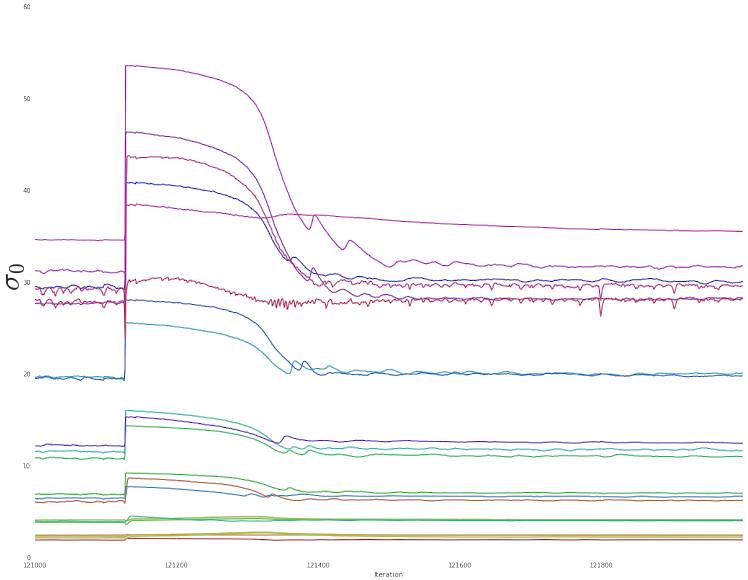
\includegraphics[width=0.48\textwidth]{images/DSpectraCloseup0aCleaned.jpg}}{(a) \discr{} $\sigma_0$}  &
\subf{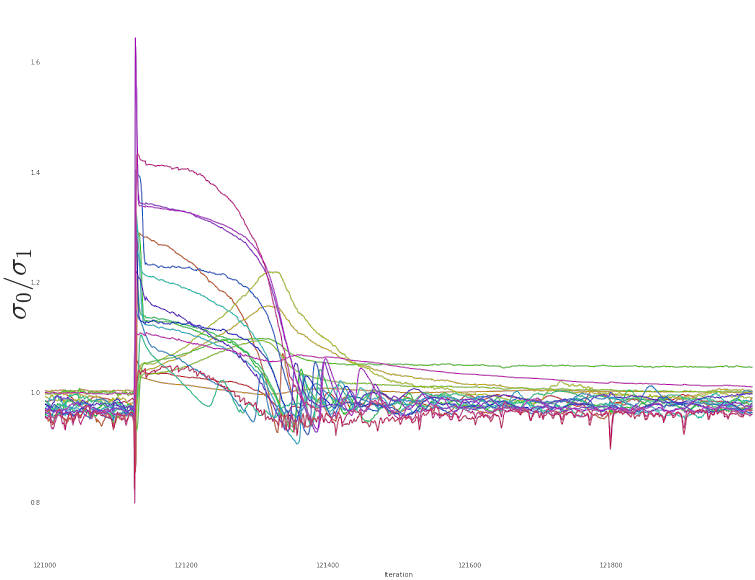
\includegraphics[width=0.48\textwidth]{images/DSpectraCloseup0bCleaned.jpg}}{(b) \discr{} $\frac{\sigma_0}{\sigma_1}$}
\end{tabular}
\caption{A closeup of \discr{}'s spectra at a noise spike.}
\label{D_spectra_closeup}
\end{figure}

If some element of \discr{}'s training process results in undesirable dynamics, it follows that the behavior of \discr{}'s spectra may hold clues as to what that element is. The top three singular values of \discr{}  differ from \gen{}'s in that they have a large noise component, tend to grow throughout training but only show a small response to collapse, and the ratio of the first two singular values tends to be centered around one, suggesting that the spectra of \discr{} have a slow decay. When viewed up close (Figure~\ref{D_spectra_closeup}), the noise spikes resemble an impulse response: at each spike, the spectra jump upwards, then slowly decrease, with some oscillation.

One possible explanation is that this behavior is a consequence of \discr{} memorizing the training data, as suggested by experiments in Section~\ref{subsec:discr_instability}.
 As it approaches perfect memorization, it receives less and less signal from real data, as both the original GAN loss and the hinge loss provide zero gradients when \discr{} outputs a confident and correct prediction for a given example. If the gradient signal from real data attenuates to zero, this can result in \discr{} eventually becoming biased due to exclusively received gradients that encourage its outputs to be negative. If this bias passes a certain threshold, \discr{} will eventually misclassify a large number of real examples and receive a large gradient encouraging positive outputs, resulting in the observed impulse responses.
 
 %...The noise in the losses of \discr{} and \gen{} (Figure~\ref{additional_stats_vanilla}(c)) could suggest another, related explanation. Spikes in the loss coincide with spikes in the spectra of \discr{}, but the magnitude of those loss spikes for \discr{} is dominated by the loss from the fake data; the upward spikes in \discr{}'s loss coincide with the downward spikes in \gen{}'s loss and have similar magnitude. This would mean that the spikes are a result of \gen{} producing a batch of images which \discr{} largely mistakes for real, resulting in a spike towards a negative bias... \andycom{I think this argument isn't invalid but it's kind of weak and it doesn't really add anything}
 
 
 %This can be seen where the upward spikes in \discr{}'s loss coinciding with the downward spikes in \gen{}'s loss and having 
 
% appears to partially agree with this interpretation-- However, the magnitude of the loss spikes is dominated by the loss from the fake data (the upward spikes in \discr{}'s loss coincide with and have similar magnitude to the downward spikes in \gen{}'s loss), which would mean that it's not a large spike towards a positive bias, but instead a large spike towards a negative bias...

 
This argument suggests several fixes. First, one might consider an unbounded loss (such as the Wasserstein loss \citep{arjovsky2017wgan}) which would not suffer this gradient attentuation. We found that even with gradient penalties and brief re-tuning of optimizer hyperparameters, our models did not stably train for more than a few thousand iterations with this loss. We instead explored changing the margin of the hinge loss as a partial compromise: for a given model and minibatch of data, increasing the margin will result in more examples falling within the margin, and thus contributing to the loss.\footnote{Unconstrained models could easily learn a different output scale to account for this margin, but the use of Spectral Normalization constrains our models and makes the specific selection of the margin meaningful.}. Training with a smaller margin (by a factor of 2) measurably reduces performance, but training with a larger margin (by up to a factor of 3) does not prevent collapse or reduce the noise in \discr{}'s spectra. Increasing the margin beyond 3 results in unstable training similar to using the Wasserstein loss. Finally, the memorization argument might suggest that using a smaller \discr{} or using dropout in \discr{} would improve training by reducing its capacity to memorize, but in practice this degrades training.




%.

%Upward spikes in D's loss also coincide with downward spikes in G's loss, and the loss term from fake data seems to dominate these spikes--could this be G overfitting to D's adversarial examples?

%-removing the bias doesn't fix this.





%One possible explanation for this behavior spikes is that \discr{} is memorizing the training data, as suggested by experiments in Section 4.2....

%-the memorization argument might suggest that using a smaller \discr{} would improve training by reducing its capacity to memorize, but in practice this degrades training.

%eventually becoming biased due to solely receiving gradients that encourage its outputs to be negative. Once this bias passes a certain threshold, \discr{} 

%-note that an unbounded loss like WGAN might not have this issue, but with our current hyperparameter settings we found WGAN unstable, even with very high R1GP values. Regardless, we believe that the tendency for \discr{} to memorize the training data is fairly general. Many previous works speculate whether or not GAN *generators* simply memorize individual samples, but this is the first time anyone has noted that \discr{} *almost certainly* memorizes samples. This may also have implications for G memorizing, since it is never directly exposed to samples so it has a hard time doing memorization, but D is directly given samples so it could memorize more easily.

%Expanding on this, we examine the spikes in \discr{}'s spectra in }. We note that, when viewed up close, these spikes

%-While this observed behavior may be partially due to the power method estimates slightly lagging the true singular values (especially if they undergo a large change), 


%-also note that sigma0/sigma1 is approximately 1--D's weights tend to be near-orthogonal? or at least, D tends to have a slow decay in svs

%

% This might partially explain why regularizing D improves stability but reduces performance, as a constrained \discr{} would be less able to memorize the training set. However, we still observe (in Section~\ref{subsec:discr_instability}) that regularized \discr{} achieve very high training accuracy and near-random test accuracy. This does not necessarily mean that regularzation fails to mollify overfitting, but suggests that this is not the primary phenomenon of interest here.


%-$^$This might also partially explain why regularizing D imparts stability but reduces performance: a constrained \discr{} is less able to overfit and memorize the training set, mollifying the effect of memorization on an undesirable output bias...yet, even with regulari

%-spikes also correlate with large loss values

%Catastrophic forgetting?

%-one other explanation would be a super-adversarial example knocks D's socks off, when G gets it just right for a batch or two and confuses the heck outta D, then it rights itself?

%-Note that even if we reset training a ton and roll the dice repeatedly so that we trundle along and avoid the huge loss spikes, collapse still occurs, so while the big spikes may play a part, they're not the only thing and avoiding them does not fix the problem.


%Noting


%if we take a model checkpoint several thousand iterations before collapse and change some hyperparameters (e.g. decay the learning rate) can


%models with different random seeds have different final singular values.

%. This begs the question of 






%-Discriminator memorization angle

%In additon 



%-applying orthogonal regularization and strongly constraining G also does not prevent collapse
%-one can go back several thousand iterations but the crash still inevitably happens
%-changing the learning rate does not prevent the crash, although if you kick the learning rate too high crash will immediately happen (even if you're switching from a learning rate which is stable to another one which is stable if you start with it)
%-If you use hierarchical latents, then the layers closest to the Z inputs are the ones that explode and many of them will explode


% We experiment with the following regularizers on D







%but that the spectra are noisy 

%We seek to impose stability through additional constraints on \discr{}.

%-Note the pathology of D's singular values: they are far noisier, with many tiny perturbations followed by oscillation. The oscillations may be artifacts of the power iterations rather than oscillations in the underlying singular values. We hypothesize this is a direct result of the adversarial training procedure: as D approaches optimality, it perfectly memorizes the real data, 

% alt: (less and less signal is provided by the real samples, resulting in D becoming biased)

%-figure showing D's singular values

%-note that imposing R1GP on D also has the effect of stabilizing G--we see that in one case the top singular value goes up and stops at a certain value. Also note that the R1GP has the odd effect of making one layer in D explodey
%-Also note that the frobenius norms grow throughout training but no matter what value we set L2 to we could not prevent collapse--maybe an adaptive L2 or a scheduled L2 is necessary.


%-Most recent papers on gan stability have focused on changing D 
%-ways we stabilize D: R1GP of various strengths, L2 on D, ortho reg (various varieties and strengths), dropout in the final feature layer (various strengths, also scheduled), output magnitude reg [cite progan]

%-we find that doing this can impart stability, but dramatically reduces performance
%-we leave our GANs unregularized and simply let them die at high performance
%-consider including the experiment where we freeze G and let D roll on, finding it to be stable, but if we freeze D and let D train on, it blows up the losses and its quality goes down the drain, highlighting the importance of discriminator optimality throughout training. Note however that we found increasing the number of D steps beyond 3 reduced performance, as did increasing D's learning rate or momentum, so there's another factor at play making it so that we can't just train D super hard and expect it to beat G constantly. \andycom{Maybe this makes memorization worse? Not sure, but let's keep speculation to a minimum if we can't back it up with evidence}

%-we note that D is dramatically overfitting to the training data--this suggests that D does not learn any sort of meaningful decision boundary between real and fake data, but instead memorizes the training set and learns a decision boundary that guides G samples to lie inside that manifold. We note that regularizing D (through data augmentation, gradient penalties, or reducing its capacity) does not change this behavior--no \discr{} we train ever has above 55\% accuracy on the ImageNet test set. \karencom{but we should note that actually that's not a problem, since D's role is to distill the data into itself and provide useful learning signal for G. We can also hypothesize that recent attempts to weight-share D with an inference net (or a classifier?) are not hugely successful because of this discrepancy in objectives.}



%\karencom{Do we need this paragraph? Maybe remove or move to Appendix}
%We seek further insight into this pathology by considering two experiments with uncollapsed models. First, we freeze \gen{} partway through training and continue to train \discr{}. In this setting, \discr{} is stable, suggesting either that \discr{} is capable of additionally memorizing the space of \gen{}'s samples, or that \discr{}'s memorization of the training set is not problematic for stability. 
%We repeat this experiment with the roles reversed, freezing \discr{} and training \gen{}. This results in immediate training collapse, with \gen{} bottoming out its loss, maxing out \discr{}'s loss, and sample quality diverging. From this, we draw two conclusions. First, as often noted in the literature, it is absolutely necessary for \discr{} to be somewhat optimal with respect to any given \gen{} in order for training to proceed. Second, training collapse does not solely stem from poor behavior in either \gen{} or \discr{}, but from their interactions in the adversarial training process. The success of methods which target \discr{}'s conditioning can arguably be understood from this point of view: so long as \discr{} is constrained and near-optimal, it provides gradients which keep \gen{} well-behaved, and render \gen{} unable to induce collapse.


%-This leads to the following conclusion/posit/supposition/hypothesis: Regardless of G's conditioning, the consequence of G winning the game is immediate and dramatic training collapse. It follows that D must remain optimal throughout training to prevent G from doing this, and that the gradients that flow from D should be constrained to prevent G from being able to adversarially annihilate the whole kit and kaboodle.

%Previous works have argued for conditioning and keeping D optimal based on the need to provide good gradients everywhere (non saturation) but have not... -this is in contrast to previous works which argue that the optimality of the discriminator is necessary in order for the gradients to G to be good? I guess that's still what we're seeing, if D is not optimal then its gradients are incorrect and G will follow a bad path and go unstable


%-stability requires optimal D, and G will break the game given the chance. it follows that it is necessary to ensure the conditioning of D is good in some sense--since regardless of g's conditioning, g will always 

%We posit that the poor conditioning we observe is a symptom



% suggesting that even if \discr{} is memorizing the training set, this 

% If this behavior is the source of instability, we might expect that training \discr{} alone with a frozen \gen{}

% given the capacity of our models, it is reasonable to suspect overfitting, but what does that actually mean here?

% We illuminate, investigate, study the effects, consequences
% We test this hypothesis by considering two experiments with uncollapsed models. First, we freeze \gen{} partway through training and continue to train \discr{}. In this setting, \discr{} is stable


% -however in the other test that's not the case--D is perfectly stable when G is not trained

% -experiment: Freeze G, D is stable, freeze D, G is stable
% -Conclusion: instability comes not from G or from D alone, but explicitly from their interaction

%The consequences of this behavior are further illuminated by the following experiment


%To further illuminate this behavior, we





%---describe experiments where we freeze G and where we freeze D






%  damping the oscillations and [enforcing stability] \andycom{awk, fix}



% This behavior indicates that while the primary symptoms of training collapse appear suddenly and sharply, other early indicators are present long before. We find that even if a training run is reset to a checkpoint thousands of iterations before collapse (with a new random seed governing noise samples and data sampling), collapse still occurs at approximately the same iteration. Freezing the first linear layer or modifying learning rates does not prevent this--another early layer will explode instead.

% This is also consistent with our observation that even if a training run is reset to a checkpoint thousands of iterations before collapse, collapse will still occur at approximately the same iteration and level of performance.

%\andycom{we suspect it's either the first singular value or the ratio of the first singular value which explode}. This may also explain why even if one resets to a checkpoint thousands of iterations before collapse, collapse will occur at approximately the same performance and iteration. % The last sentence may need to be rearranged and stuck elsewhere

%-enforcing very strong conditioning (summed ortho2) on G results in all singular values being 1, but doesn't prevent a crash; we conclude that while \gen{} conditioning is *necessary* for GAN stability, it is not *sufficient* and turn our attention to \discr{}


% -we also tried regularizing these quantities instead of clamping them, with similar results

% Even with very strong orthogonal regularization applied to \gen{} (setting all singular values to $1$ throughout training and enforcing a fixed Frobenius norm), collapse still occurs.



% junk paragraphs rewrite bro
%One possible explanation for these spikes is that \discr{} is memorizing the training data, and as it approaches optimality it receives less and less signal from real data, eventually becoming biased due to solely receiving gradients that encourage its outputs to be negative. Once this bias passes a certain threshold, \discr{} 

%-one other explanation would be a super-adversarial example knocks D's socks off, when G gets it just right for a batch or two and confuses the heck outta D, then it rights itself?

%-Note that even if we reset training a ton and roll the dice repeatedly so that we trundle along and avoid the huge loss spikes, collapse still occurs, so while the big spikes may play a part, they're not the only thing and avoiding them does not fix the problem.